%%%%%%%%%%%%%%%%%%%%%%%%%%%%%%%%%%%%%%%%%
% University/School Laboratory Report
% LaTeX Template
% Version 3.1 (25/3/14)
%
% This template has been downloaded from:
% http://www.LaTeXTemplates.com
%
% Original author:
% Linux and Unix Users Group at Virginia Tech Wiki 
% (https://vtluug.org/wiki/Example_LaTeX_chem_lab_report)
%
% License:
% CC BY-NC-SA 3.0 (http://creativecommons.org/licenses/by-nc-sa/3.0/)
%
%%%%%%%%%%%%%%%%%%%%%%%%%%%%%%%%%%%%%%%%%

%----------------------------------------------------------------------------------------
%	PACKAGES AND DOCUMENT CONFIGURATIONS
%----------------------------------------------------------------------------------------

\documentclass{article}

\usepackage[version=3]{mhchem} % Package for chemical equation typesetting
\usepackage{siunitx} % Provides the \SI{}{} and \si{} command for typesetting SI units
\usepackage{graphicx} % Required for the inclusion of images
\usepackage{natbib} % Required to change bibliography style to APA
\usepackage{amsmath} % Required for some math elements 
\usepackage{enumerate} % Required for the enumerate function
\usepackage[americanvoltages,siunitx]{circuitikz} % Required for the drawing of circuit diagrams
\usepackage{caption}
\usepackage{graphicx}
\usepackage{subcaption}
\usepackage{xfrac}
\usepackage{float}
\usepackage{enumitem}
\usepackage{epstopdf}
\usepackage{booktabs}
\usepackage[]{mcode}
\usepackage{tikz}
\usetikzlibrary{shapes,arrows}
\usepackage{verbatim}

\setlength\parindent{0pt} % Removes all indentation from paragraphs

\renewcommand{\labelenumi}{\alph{enumi}.} % Make numbering in the enumerate environment by letter rather than number (e.g. section 6)

%\usepackage{times} % Uncomment to use the Times New Roman font

\graphicspath{{./fig/}}

%----------------------------------------------------------------------------------------
%	DOCUMENT INFORMATION
%----------------------------------------------------------------------------------------

\title{Systems Modelling \& Control \\ Lab 1 \\ ENG325} % Title

\author{Shane \textsc{Reynolds}} % Author name

\date{\today} % Date for the report

\begin{document}

\maketitle % Insert the title, author and date

\begin{center}
\begin{tabular}{l r}
Date Performed: & March 25, 2016 \\ % Date the experiment was performed
Instructor: & Damien Hill % Instructor/supervisor
\end{tabular}
\end{center}

% If you wish to include an abstract, uncomment the lines below
% \begin{abstract}
% Abstract text
% \end{abstract}

%----------------------------------------------------------------------------------------
%	SECTION 1
%----------------------------------------------------------------------------------------

\section{Objective}

To evaluate the accuracy of a linearised mathematical model applied to a non-linear pump tank system, with parameters derived from experimental data.

\section{Background}

The pump tank system is illustrated in Figure 1. The input voltage to the pump is denoted by $U(t)$. The input and output flow are denoted as $Q_i$ and $Q_o$ respectively. The height of the head in the cylindrical tank is measured by a sensor inside the tank. The sensor reports a voltage $HU(t)$. When in operation the system is at a steady state for some given input voltage $U(t)$. Changes to the input of the system $U(t)$ cause a change in the operation of the pump which causes the input flow rate to the tank $Q_i$ to change. The system output $HU(t)$ undergoes a transient response to the change in the input signal until it eventually reaches a new steady state.

% Draw a simple picture of the pump tank system use this section to calculate the cross sectional area of the device.
\tikzstyle{block} = [draw, fill=blue!20, rectangle, 
minimum height=3em, minimum width=6em]
\tikzstyle{sum} = [draw, fill=blue!20, circle, node distance=1cm]
\tikzstyle{input} = [coordinate]
\tikzstyle{output} = [coordinate]
\tikzstyle{pinstyle} = [pin edge={to-,thin,black}]

% The block diagram code is probably more verbose than necessary
\begin{figure}[H]
	\centering
	\caption{Pump Tank Fluid System}
	\begin{tikzpicture}[auto, node distance=2cm,>=latex']
	% We start by placing the blocks
	\node [block, name=pump, pin={[pinstyle,pin edge={<-}]above:$U(t)$}]{Pump};
	\node [block, right of=pump, node distance=3cm, pin={[pinstyle,pin edge={->}]above:$HU(t)$}](tank){Tank};
	\draw[->] (pump) -- node [name=u] {$Q_i$} (tank);
	\node [block, below of=u] (reservoir){Reservoir};
	\node [name=t, right of=tank]{};
	\node [name=v, below of=t]{};
	\draw[->] (tank) -- node [name=z] {$Q_o$}(tank-|v) |- (reservoir);
	\node [name=a, left of=pump]{};
	\draw[->] (reservoir) -- (reservoir -| a) |- (pump);
	\end{tikzpicture}
\end{figure}


% Talk about the general derivation of the model which explains the system.
To derive a general model which takes an input of pump voltage $U(t)$ and an output of the sensor voltage $HU(t)$, we begin by considering the volume of the tank. The volume of the tank for some small time perturbation $\delta t$ is given by:
\begin{align}
	V(t + \delta t) = A\big(H(t + \delta t) + dH(t + \delta t)\big)
\end{align}

The variable $A$ is the cross sectional area of the tank, which is constant with respect to time. The function $H(t)$ is the operating point for the head of the tank and the function $dH(t)$ represents small perturbations in the head about the large bias signal $H(t)$. Now if the both the input flow and output flow to the tank are also broken up into a bias point and small signal representation we get the following functions respectively: $Q_i$, $dQ_i$, $Q_o$ and $dQ_o$. We can then write equation (1) as:
\begin{align}
	A\big(H(t + \delta t) + dH(t + \delta t)\big) &= A\big(H(t) + dH(t)\big) + \big((Q_i + dQ_i) - (Q_o + dQ_o)\big) \delta t \nonumber
\end{align}

Rearranging this we get the following expression:
\begin{align}
	A\bigg(\frac{H(t + \delta t) - H(t)}{\delta t} + \frac{dH(t + \delta t) - dH(t)}{\delta t}\bigg) = (Q_i - Q_o) + (dQ_i - dQ_o) \nonumber
\end{align}

In the limit as $\delta t \rightarrow 0$ we get the following expression:
\begin{align}
	A\bigg(\frac{dH(t)}{dt} + \frac{d}{dt}\big(dH(t)\big)\bigg) = (Q_i - Q_o) + (dQ_i - dQ_o)
\end{align}

At this point we consider to the large signal and small signal models independently. Assuming the model is linear we can look at each section independently and use superposition to arrive at an expression for our final model. From equation (2) consider the large signal model:
\begin{align}
	A\bigg(\frac{dH(t)}{dt}\bigg) = Q_i - Q_o  \nonumber
\end{align}

At steady state the rate of change in the head is equal to zero since $Q_i= Q_o$. Trivially, we see that $H(t) = C_1$, where $C_1$ is a constant. If we let $H(0) = H_o$, where $H_o$ is the bias point, then $C_1 = H_o$. Hence, we get the following expression:
\begin{align}
	H(t) = H_o
\end{align}

The small signal model is slightly more involved. From equation (2) consider the small signal model:
\begin{align}
	A\bigg(\frac{d}{dt}\big(dH(t)\big)\bigg) = dQ_i - dQ_o \nonumber
\end{align}

According to Ogata (1998) the resistance of a fluid system is given by the change in the level difference in the tank head divided by the change in the flow rate. Mathematically, this can be shown to be:
\begin{align}
	R = \frac{dH}{dQ} \nonumber
\end{align}

Rearranging yields:
\begin{align}
dQ = \frac{dH}{R_t}
\end{align}

Ogata also defines tank capacitance $C$ as the change in the stored liquid divided by the change in the head - in a tank with constant cross sectional area this value is equal to the cross sectional area of the tank, $A$. The function which represents $dQ_o$ is non-linear. Replacing $dQ_o$ with equation (4) linearises the model. Further, replacing $A$ with $C$ yields the following expression:
\begin{align}
\frac{d}{dt}\big(dH(t)\big) &= \frac{1}{C}dQ_i - \frac{1}{R_{t}C}dH(t)
\end{align}

Solving this equation, we get the following integral:
\begin{align}
dH(t) = \int_{0}^{t}\frac{1}{C}dQ_i - \frac{1}{R_{t}C}dH(\tau) d\tau
\end{align}

Finally, using the principal of superposition with expressions (3) and (6), the actual head in the tank, say $H_{tot}(t)$, is given by the equation:
\begin{align}
H_{tot}(t) 	&= H(t) + dH(t) \nonumber \\
&= H_o + \int_{0}^{t}\frac{1}{C}dQ_i - \frac{1}{R_{t}C}dH(\tau) d\tau
\end{align}

In our tank system, assuming turbulent flow at the outlet valve, $Q_o = K_t\sqrt{H}$ (Ogata, 1998). From this equation we obtain:
\begin{align}
	dQ_o = \frac{K_t}{2\sqrt{H}}dH \nonumber
\end{align}

It follows that we can estimate the resistance of the system at some operating point $H$ and $Q_o$ with the following expression:
\begin{align}
	R_t = \frac{dH}{dQ_o} = \frac{2H}{Q_o} \nonumber
\end{align}

Noting that in the steady state $Q_o = Q_i$, we get:
\begin{align}
	R_t = \frac{2H}{Q_i}
\end{align}

\newpage

%----------------------------------------------------------------------------------------
%	SECTION 2
%----------------------------------------------------------------------------------------

\section{Derivation of the model and model parameters using experimental evidence}

\subsection{Task 1}
 
 To find an equation which linked the input pump voltage $U(t)$ to the input flow rate $Q_{i}(t)$ experimental data was collected by blocking the output valve and allowing the pump to fill the storage tank to 120mm of head at different voltages. The data is presented in Table 1.
 
 \begin{table}[H]
 	\centering
 	\caption{Experimental Data}
 	\begin{tabular}{ccc}
 		\toprule
 		$U(t)$  & $Q_{i}(t)$ & $t$ \\
 		($\si{\volt}$) & ($\si{\milli\meter\per\cubed\second}$) & ($\si{\second}$) \\\midrule
 		2.0 & 4435.91 & 7.00 \\
 		2.5 & 5645.70 & 5.50 \\
 		3.0 & 6765.00 & 4.59 \\
 		3.5 & 7821.50 & 3.97 \\
 		4.0 & 8649.41 & 3.59 \\
 		4.5 & 9466.88 & 3.28 \\\bottomrule
 	\end{tabular}
 \end{table}
 

A linear relationship between $U(t)$ and $Q_{i}(t)$ can be seen in Figure 2. Simple linear regression run on the approximately linear relationship yielded equation (9) with an R$^2$ of 0.9933.

\begin{align}
	Q_{i}(t) = 2012.71U(t) + 589.42
\end{align}


\begin{figure}[H]
	\centering
	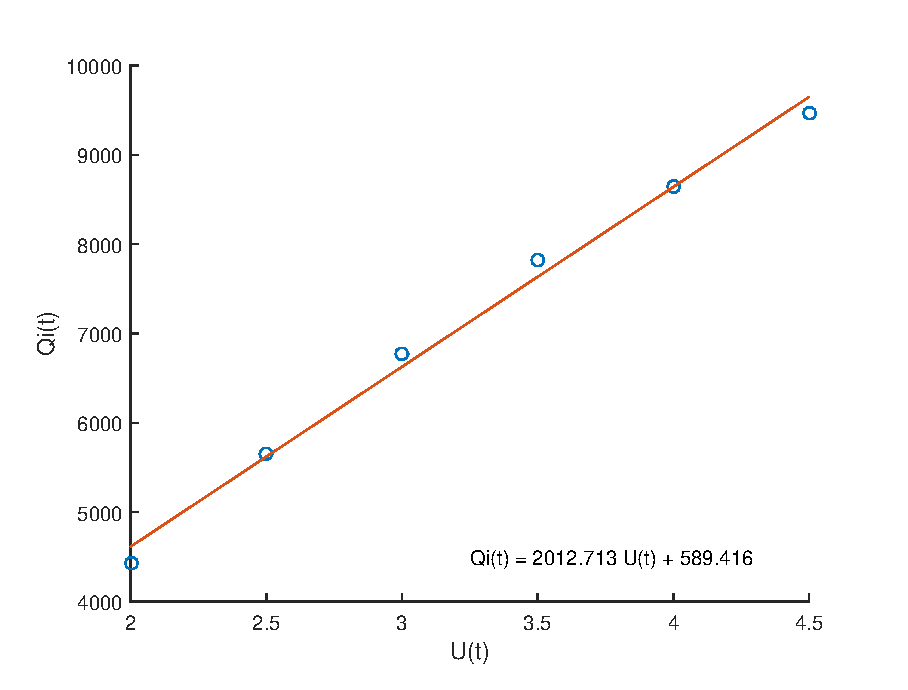
\includegraphics[scale=0.5]{fig1.eps}
	\captionof{figure}{Scatter plot of pump input voltage versus input flow rate}
\end{figure}

\subsection{Task 2}

Experimental data was collected to find an equation which linked the output sensor voltage $HU(t)$ to the actual height of water in the column tank $H(t)$. The data is presented in Table 2.

\begin{table}[H]
	\centering
	\caption{Experimental Data}
	\begin{tabular}{S[table-format=3.2] S[table-format=3.2] S[table-format=3.2]}
		\toprule
		{$U(t)$}  & {$H(t)$} & {$HU(t)$} \\
		{($\si{\volt}$)} & {($\si{\milli\meter}$)} & {($\si{\volt}$)} \\\midrule
		1.50 & \ \ 9.00 & 0.86 \\
		2.00 & \ 37.00 & 1.22 \\
		2.11 & \ 47.00 & 1.27 \\
		2.50 & \ 70.00 & 1.63 \\
		2.70 & \ 92.00 & 1.85 \\
		3.00 & 110.50 & 2.23 \\
		3.20 & 136.00 & 2.65 \\
		3.50 & 159.00 & 3.28 \\\bottomrule
	\end{tabular}
\end{table}

A linear relationship between $HU(t)$ and $H(t)$ can be seen in Figure 3. Simple linear regression run on the approximately linear relationship yielded equation (10) with an R$^2$ of 0.9760.

\begin{align}
HU(t) = 0.0155H(t) + 0.589
\end{align}


\begin{figure}[H]
	\centering
	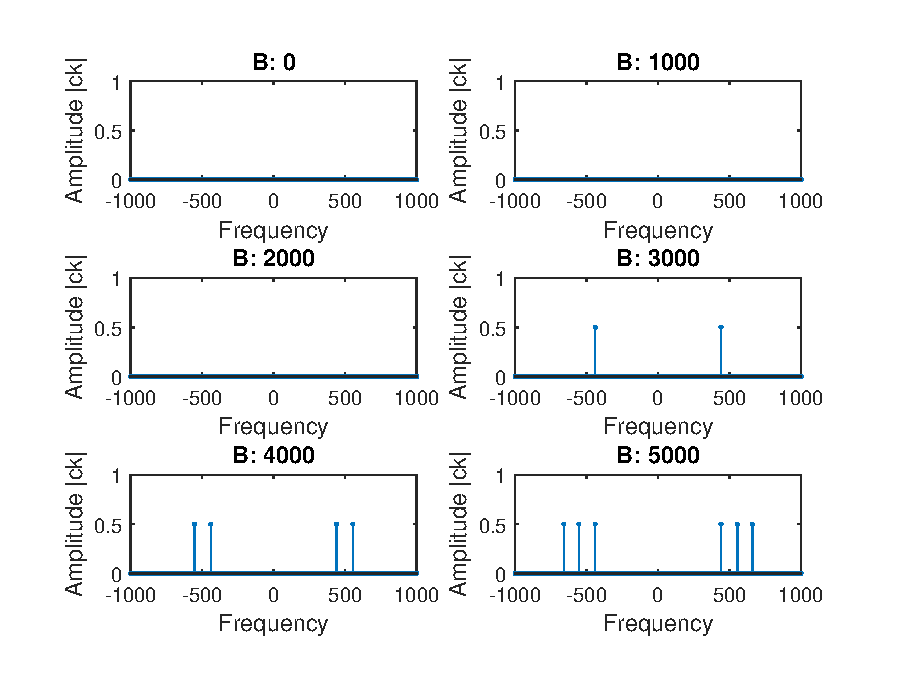
\includegraphics[scale=0.5]{fig2.eps}
	\captionof{figure}{Scatter plot of head in column tank versus sensor output voltage}
\end{figure}

\subsection{Task 3}

Experimental data was collected for the device in steady state around three different operating points: 25\%, 50\% and 75\% of the tank volume. Using equation (8) we can find that the output resistance, assuming turbulent flow, for each of the operating points. Additionally, the capacitance is simply the cross sectional area of the tank $A$. The data is presented in Table 3.

\begin{table}[H]
	\centering
	\caption{Experimental Data}
	\begin{tabular}{c S[table-format=3.2] S[table-format=3.2] S[table-format=3.2] S[table-format=3.2] S[table-format=3.2]}
		\toprule
		Operating Point & {$U(t)$}  & {$H(t)$} & {$HU(t)$} & $R$ & $C$ \\
		 & {($\si{\volt}$)} & {($\si{\milli\meter}$)} & {($\si{\volt}$)} & {($\si{\second\per\milli\meter\squared}$)} & {($\si{\milli\meter\squared}$)} \\\midrule
		25\% & 2.11 & \ 47.00 & 1.27 & 0.0194 & 258.76 \\
		50\% & 2.70 & \ 92.00 & 1.85 & 0.0305 & 258.76 \\
		75\% & 3.20 & 136.00 & 2.65 & 0.0386 & 258.76 \\\bottomrule
	\end{tabular}
\end{table}

\subsection{Task 4}

Each of the 3 operating points shown in Table 3 above yield their own linearised differential equations and hence we get a different expression for $H_{tot}(t)$ at each of the 3 operating points.\\

For the operating point at 25\% we get the differential equation:
\begin{align}
	\frac{d}{dt}\big(dH(t)\big) &= \frac{1}{258.76}dQ_i - \frac{1}{0.0194 \times 258.76}dH(t) \nonumber
\end{align}

This gives us the expression:
\begin{align}
	H_{tot}(t) = H_o + \int_{0}^{t}\frac{1}{258.76}dQ_i - \frac{1}{0.0194\times 258.76}dH(\tau) d\tau \nonumber
\end{align}
\hspace{1.5cm}

Similarly the differential equation and susbsequent expression for $H_{tot}(t)$ for the 50\% operating bias point is:
\begin{align}
\frac{d}{dt}\big(dH(t)\big) &= \frac{1}{258.76}dQ_i - \frac{1}{0.0305 \times 258.76}dH(t) \nonumber
\end{align}

And the expression:
\begin{align}
H_{tot}(t) = H_o + \int_{0}^{t}\frac{1}{258.76}dQ_i - \frac{1}{0.0305\times 258.76}dH(\tau) d\tau \nonumber
\end{align}

\newpage

Finally, for the 75\% operating bias point, we get:
\begin{align}
\frac{d}{dt}\big(dH(t)\big) &= \frac{1}{258.76}dQ_i - \frac{1}{0.0386 \times 258.76}dH(t) \nonumber
\end{align}

Which gives the expression:
\begin{align}
H_{tot}(t) = H_o + \int_{0}^{t}\frac{1}{258.76}dQ_i - \frac{1}{0.0386 \times 258.76}dH(\tau) d\tau \nonumber
\end{align}


%----------------------------------------------------------------------------------------
%	SECTION 3
%----------------------------------------------------------------------------------------

\section{Simulation}

\subsection{Task 5}
Data was collected for a total time period of 80 seconds during which time the input voltage for the pump was set to 2$\si{\volt}$ and then, once the system had stabilised after about 5 seconds, the voltage was stepped up to 3 $\si{\volt}$. Data was collected until the system had stabilised again.

\subsection{Task 6}
An approximation of a system described by a first order differential equation can be found by discritising the temporal dimension of the system and using a Euler approximation for the derivative. Applying this to the general differential equation (5), we get the following:
\begin{align}
	\frac{dH_{n+1} - H_n}{\Delta t} = \frac{1}{C}dQ_i - \frac{1}{R_{t}C}dH_n \nonumber
\end{align}

The discretised model simplifies to:
\begin{align}
	dH_{n+1} = dH_{n} + \frac{\Delta t}{C} \big(dQ_i - \frac{1}{R_{t}}dH_n\big)
\end{align}

Applying the simulation at the 50\% bias point using 0.01 second time steps, the simulation model (11) becomes:
\begin{align}
dH_{n+1} = dH_{n} + \frac{0.01}{258.76} \big(dQ_i - \frac{1}{0.0305}dH_n\big)
\end{align}

% Talk about how the model was implemented.
The real world non-linear data captured from experiments includes both the large and small signals, that is $H_{tot}(t) = H_o + dH(t)$. The simulation model in equation (12), however, will only report the cumulation of $dH(t)$. So that the simulated model output can be compared with the real world data, each real world data point will undergo the following transformation: $dH = H_{tot} - H_o$, where $H_o$ is the steady state condition prior to the step change in the input voltage $U(t)$.\\

The simulation model was implemented in Matlab with code that can be seen in Appendix A. The results from the simulation can be seen in Figure 4. Additionally the absolute error was plotted versus time to provide better insight on the model accuracy.

\begin{figure}[H]
	\centering
	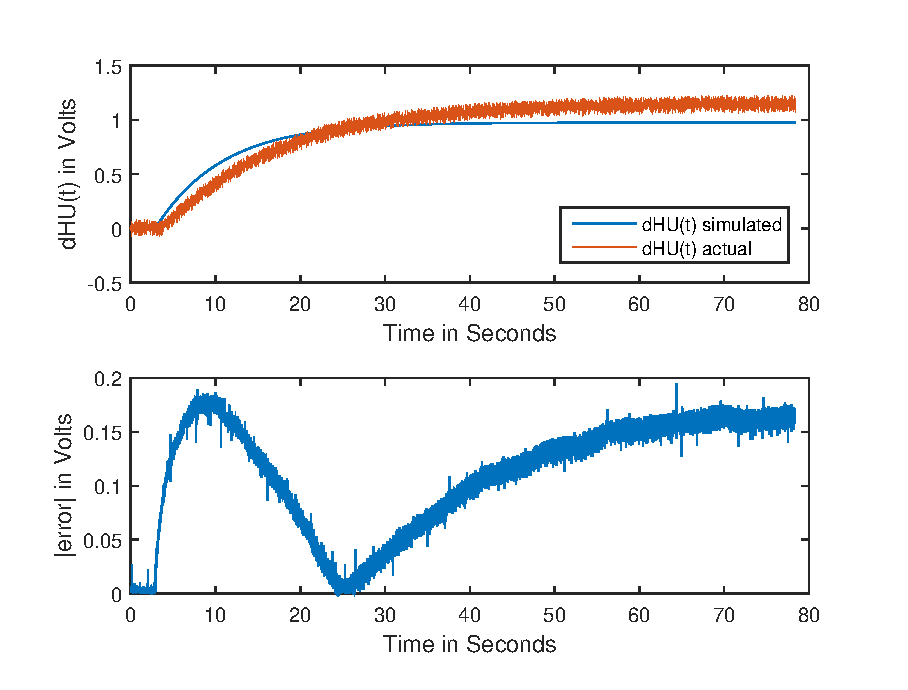
\includegraphics[scale=0.8]{fig3.eps}
	\captionof{figure}{Scatter plot of head in column tank versus sensor output voltage}
\end{figure}

%----------------------------------------------------------------------------------------
%	SECTION 3
%----------------------------------------------------------------------------------------

\section{Evaluation of the results}

\subsection{Task 7}
The simulation of the non-linear tank system performed quite poorly, however, the absolute error present in the simulation seems to be bounded to 0.2V. Error this large is most likely due to model misspecification or errors in the estimated model parameters. Mitigation of this error would require a correct model specification and correctly estimated model parameters, however, there is some error that can not be eliminated which may be attributed to two factors present in the implementation of the simulated model.\\

The first source of error is due to the linearisation of the non-linear model. The process of linearisation replaces non-linear elements of the model with linear elements and assumes that the model will only be used to assess small variations about some specified operating point. The 50\% operating point was the bias point around which the simulation was run, however, the actual system started closer to the 25\% bias point. It would be expected that some error is present at the start of the model simulation and again at the end of the simulation, where the linear model would diverge with the actual non-linear model most noticeably. This effect can be seen in Figure 4 in the absolute error plot.\\

The second source of error comes from the discretisation of the temporal dimension with the implementation of Euler's method of approximation. Euler's approximation in general states that for some small perturbation $h$, the approximate solution to the first order differential equation $\frac{dy}{dt} = f(y,t)$ is given by the following:
\begin{align}
	y_{n+1} = y_n + hf(y,t) 
\end{align}

Consider the Taylor series expansion derivation of this numerical scheme about some fixed point $t_0$:
\begin{align}
	y(t_0+h) 	&= y(t_0) + h\frac{dy(t_0)}{dt} + O(h^2) \nonumber \\
				&\approx y(t_0) + h\frac{dy(t_0)}{dt} \nonumber
\end{align}

Now since $\frac{dy}{dt} = f(y,t)$, then:
\begin{align}
	y(t_0+h) \approx y(t_0) + hf(y(t_0),t_0)
\end{align}

The higher order terms $O(h^2)$ have been truncated in the Euler approximation scheme shown in equation (14). This means that for each time step we take there is a small amount of error which is cumulatively added to the model. In some instances, the error can grow without bound, which causes the simulation to blow up. Fortunately, in this case, the error appears to be bounded, however, it would account for a small amount of the deviation of the simulated results to the actual results.

\newpage

\subsection{Task 8}

The simulation model was run a second time in order to compare the performance of the models around all three operating points 25\%, 50\% and 75\%. The implementation of this code can be seen in Appendix B. The results from the simulation can be seen in Figure 5. The differences between the models lay solely in the resistor values at each of the three operating points. These different resistor values affect the time constant of the solution to the first order system. The final asymptotic levels which each of the plots appear to approach are indicative of the different steady states of the system in response to a 1V step in the input.

\begin{figure}[H]
	\centering
	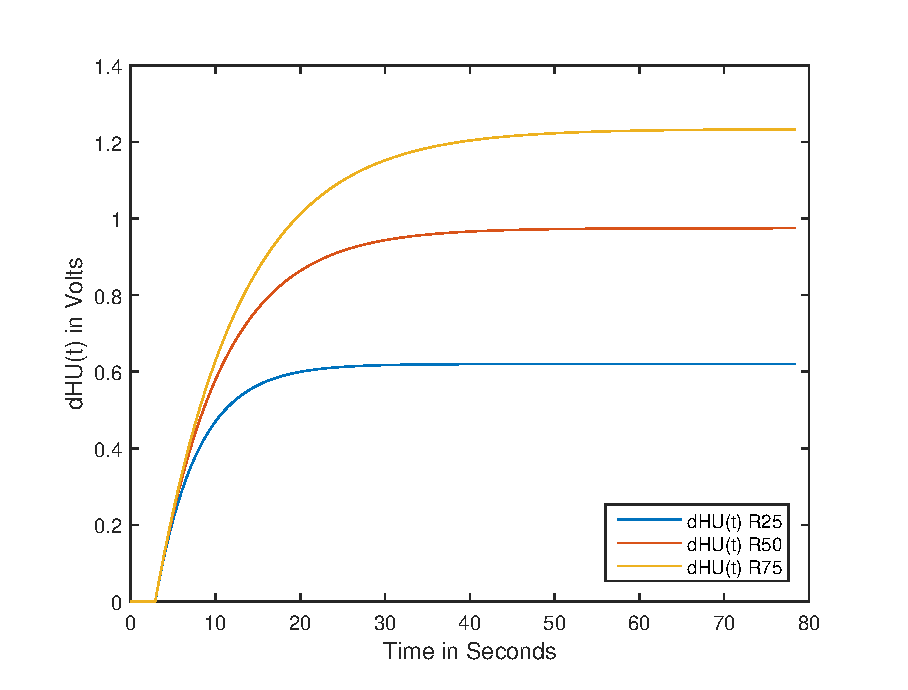
\includegraphics[scale=0.8]{fig4.eps}
	\captionof{figure}{Scatter plot of head in column tank versus sensor output voltage}
\end{figure}

%----------------------------------------------------------------------------------------
%	BIBLIOGRAPHY
%----------------------------------------------------------------------------------------

\section{References}

Ogata, K. (1998). \textit{System Dynamics 4th Edn}. Pearson.

\newpage

%----------------------------------------------------------------------------------------
%	APPENDIX
%----------------------------------------------------------------------------------------

\section{Appendices}

\subsection{Appendix A}
Implementation of simulation using Matlab:
\begin{lstlisting}
%%%%%%%%%%%%%%%%%%%%%%%%%%%%%%%%%%%%%%%%%%%%%%%%%%%%%%%%%%%%%%%%%%%%%%%%%%
% This script runs a simulation on a single tank with an output valve
% and an input valve which is driven by an electric pump. The simulation
% has been implemented using Euler approximation.
%%%%%%%%%%%%%%%%%%%%%%%%%%%%%%%%%%%%%%%%%%%%%%%%%%%%%%%%%%%%%%%%%%%%%%%%%%

% Load system data and specify variables
filepath = 'C:\Users\Shane Reynolds\Desktop\Lab 1 Data\Lab 1 Data\step1.txt';
data = textread(filepath);
time = data(1:end,1);
dataHo = 1.293;
datahu = data(1:end,3) - dataHo;

% Specify time step size and storage for simulation output
dt = 0.01;
hu = [0];

% Specify simulation model parameters
C = pi*((18.7)^2 - 2*(3.18)^2)/4;
R = 0.0305;

% Run simulation
for i = 1:(size(data(1:end,2))-1)
	if data(i,2) == 2
		hu(i+1) = 0;
	else
		hu(i+1) = hu(i) + (dt/C)*(31.97 - (1/R)*hu(i));
	end
end

% Plot simulated and acutal data on same plot
subplot(2,1,1)
plot(time,hu)
hold on
plot(time,data(1:end,3)-1.287)
xlabel('Time in Seconds')
ylabel('dHU(t) in Volts')
legend('dHU(t) simulated','dHU(t) actual',...
'Location','southeast')

% Plot absolute error
subplot(2,1,2)
error = abs(datahu' - hu);
plot(time,error)
xlabel('Time in Seconds')
ylabel('|error| in Volts')
\end{lstlisting}

\newpage

\subsection{Appendix B}

\begin{lstlisting}
%%%%%%%%%%%%%%%%%%%%%%%%%%%%%%%%%%%%%%%%%%%%%%%%%%%%%%%%%%%%%%%%%%%%%%%%%%
% This script runs a simulation on a single tank with an output valve
% and an input valve which is driven by an electric pump. The simulation
% has been implemented using Euler approximation for resistor values
% around the 25, 50 and 75 percent bias points.
%%%%%%%%%%%%%%%%%%%%%%%%%%%%%%%%%%%%%%%%%%%%%%%%%%%%%%%%%%%%%%%%%%%%%%%%%%
	
% Specify time step size and storage for simulation output
dt = 0.01;
hu = [0 0 0];
	
% Specify simulation model parameters
C = pi*((18.7)^2 - 2*(3.18)^2)/4;
R25 = 0.0194;
R50 = 0.0305;
R75 = 0.0386;
	
% Run simulation
for i = 1:(size(data(1:end,2))-1)
	if data(i,2) == 2
		hu(i+1,1:end) = 0;
	else
		hu(i+1,1) = hu(i,1) + (dt/C)*(31.97 - (1/R25)*hu(i,1));
		hu(i+1,2) = hu(i,2) + (dt/C)*(31.97 - (1/R50)*hu(i,2));
		hu(i+1,3) = hu(i,3) + (dt/C)*(31.97 - (1/R75)*hu(i,3));
	end
end
	
% Plot simulated data on same plot
plot(time,hu(1:end,1))
hold on
plot(time,hu(1:end,2))
plot(time,hu(1:end,3))
xlabel('Time in Seconds')
ylabel('dHU(t) in Volts')
legend('dHU(t) R25','dHU(t) R50', 'dHU(t) R75',...
'Location','southeast')
\end{lstlisting}

%----------------------------------------------------------------------------------------


\end{document}